\section{Wie kann ich etwas Drucken?}
{
\usebackgroundtemplate{%
\colorbox{BackgroundJGH}{%
\vbox to \paperheight{\vfil\hbox to \paperwidth{\hfil
\includegraphics[width=\paperwidth]{images/steps/base.png}\hfil}\vfil}
}
}
\begin{frame}
  \frametitle{Wie kann ich etwas Drucken?}
\end{frame}
}
{
\usebackgroundtemplate{%
\colorbox{BackgroundJGH}{%
\vbox to \paperheight{\vfil\hbox to \paperwidth{\hfil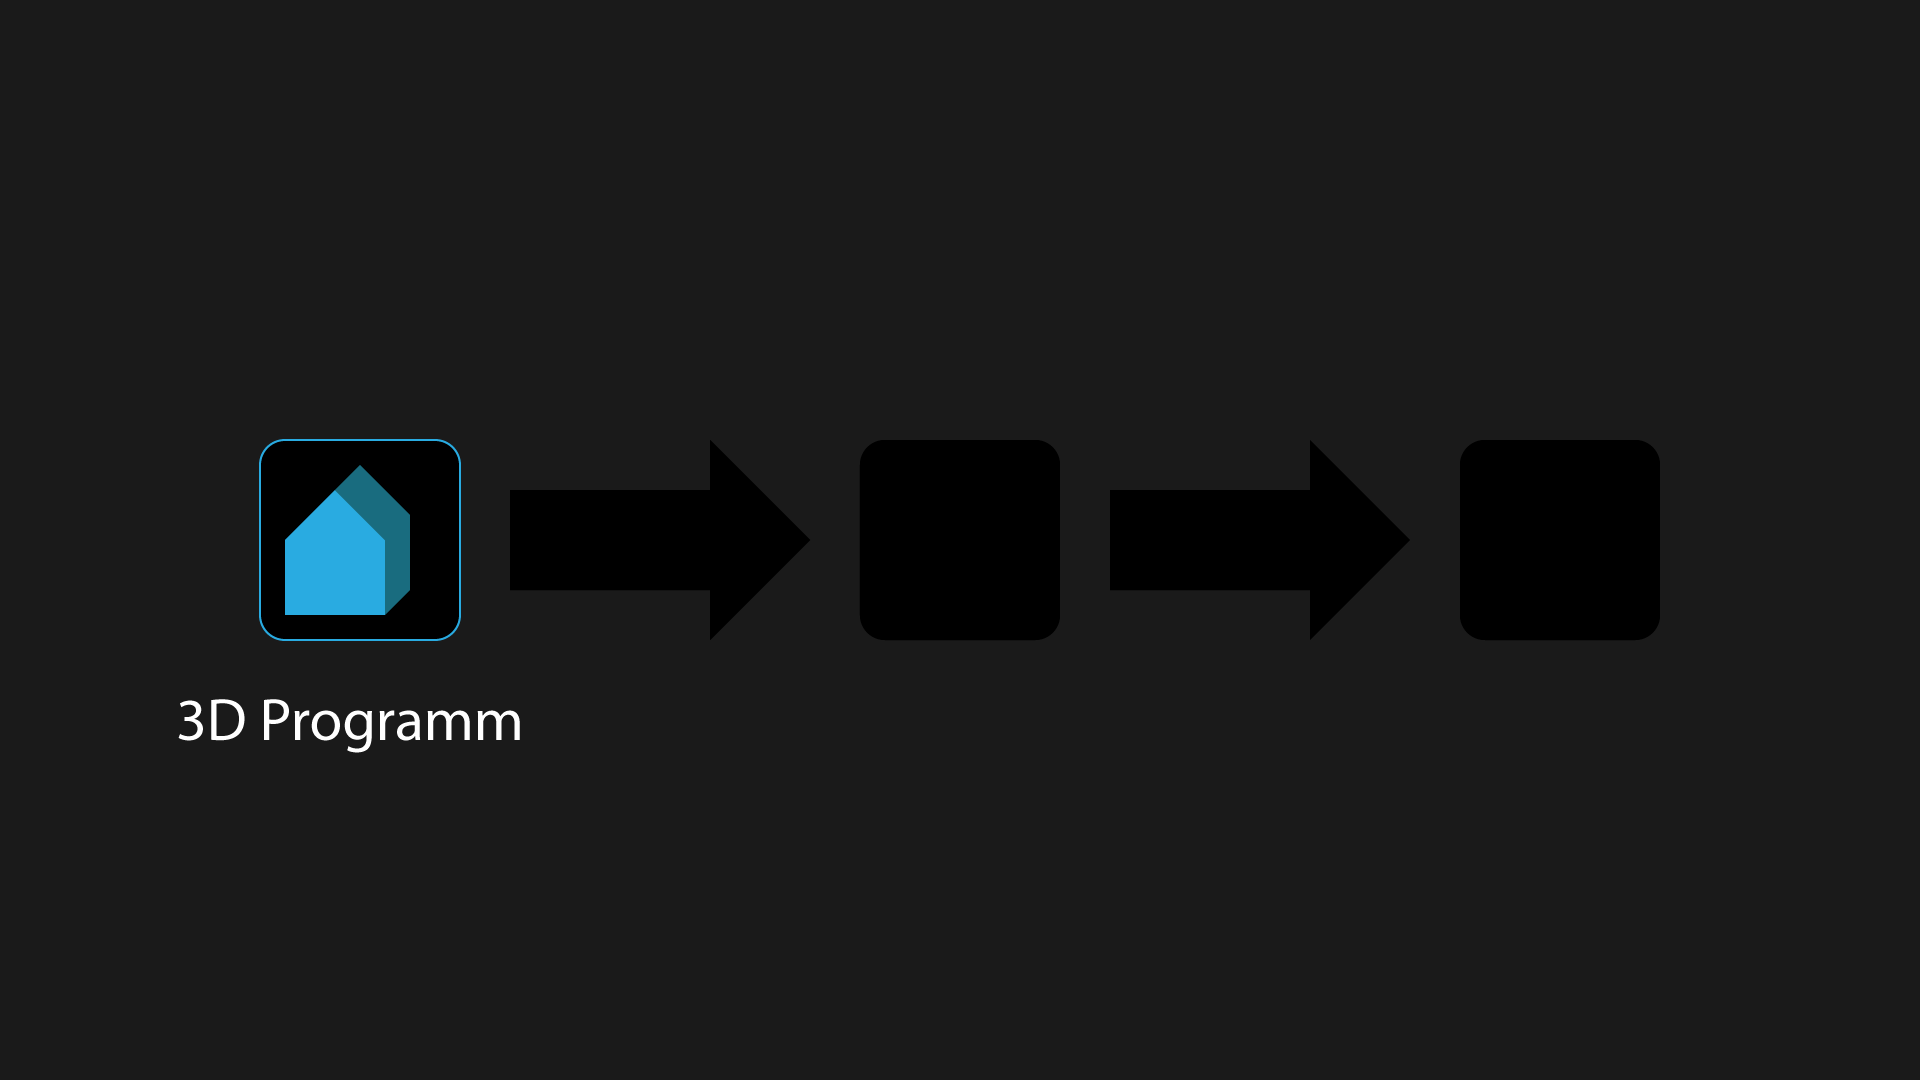
\includegraphics[width=\paperwidth]{images/steps/3d_prog.png}\hfil}\vfil}
}
}
\begin{frame}
  \frametitle{3D Programm}
\end{frame}
}

{
\usebackgroundtemplate{%
\colorbox{BackgroundJGH}{%
\vbox to \paperheight{\vfil\hbox to \paperwidth{\hfil
\includegraphics[width=\paperwidth]{images/steps/3d_prog_bg.png}\hfil}\vfil}
}
}
\begin{frame}
  \frametitle{3D Programm}
  \begin{itemize}
    \item Modelierungsprogramm \pause
    \begin{itemize}
      \item Blender \pause
    \end{itemize}
    \item CAD Programm \pause
    \begin{itemize}
      \item FreeCAD \pause
    \end{itemize}
    \item Objektbibliothek \pause
    \begin{itemize}
      \item Thingiverse
    \end{itemize}
  \end{itemize}
\end{frame}
}
{
\usebackgroundtemplate{%
\colorbox{BackgroundJGH}{%
\vbox to \paperheight{\vfil\hbox to \paperwidth{\hfil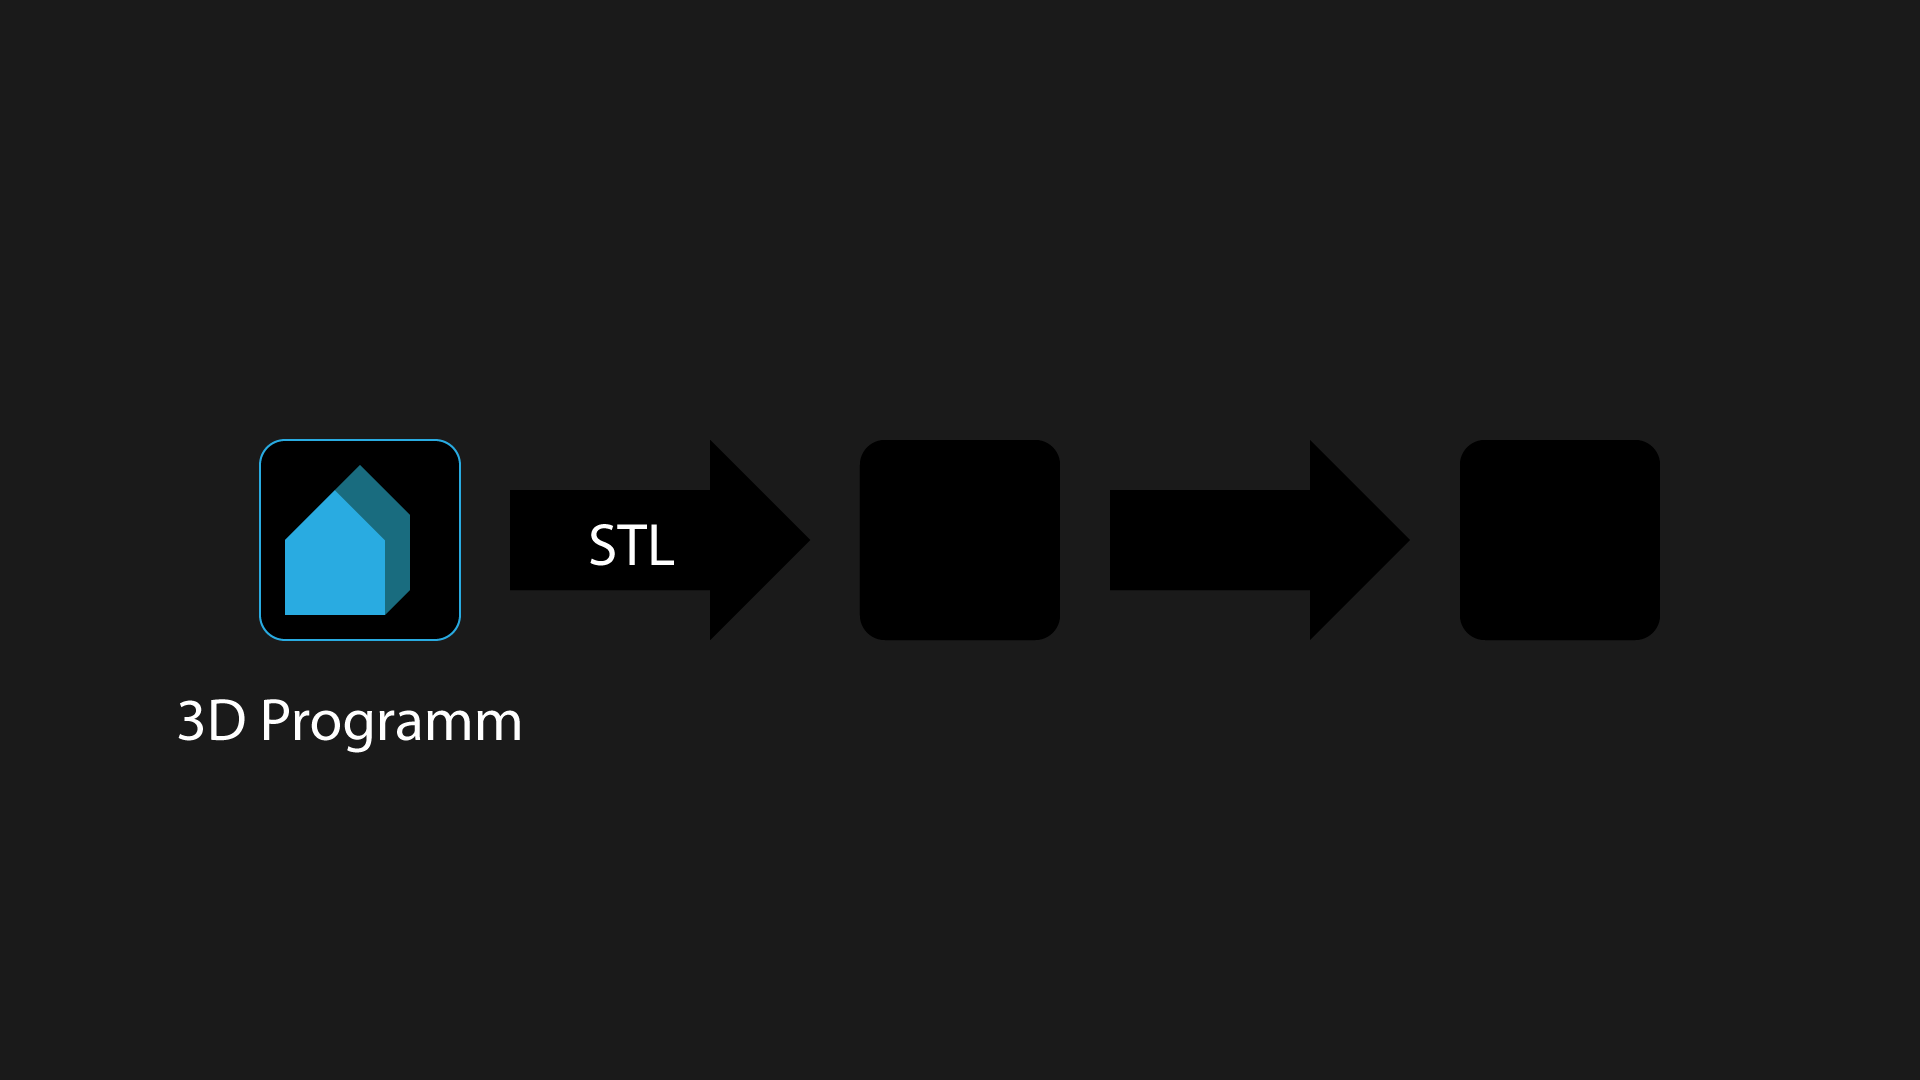
\includegraphics[width=\paperwidth]{images/steps/stl.png}\hfil}\vfil}
}
}
\begin{frame}
  \frametitle{STL Datei}
\end{frame}
}
{
\usebackgroundtemplate{%
\colorbox{BackgroundJGH}{%
\vbox to \paperheight{\vfil\hbox to \paperwidth{\hfil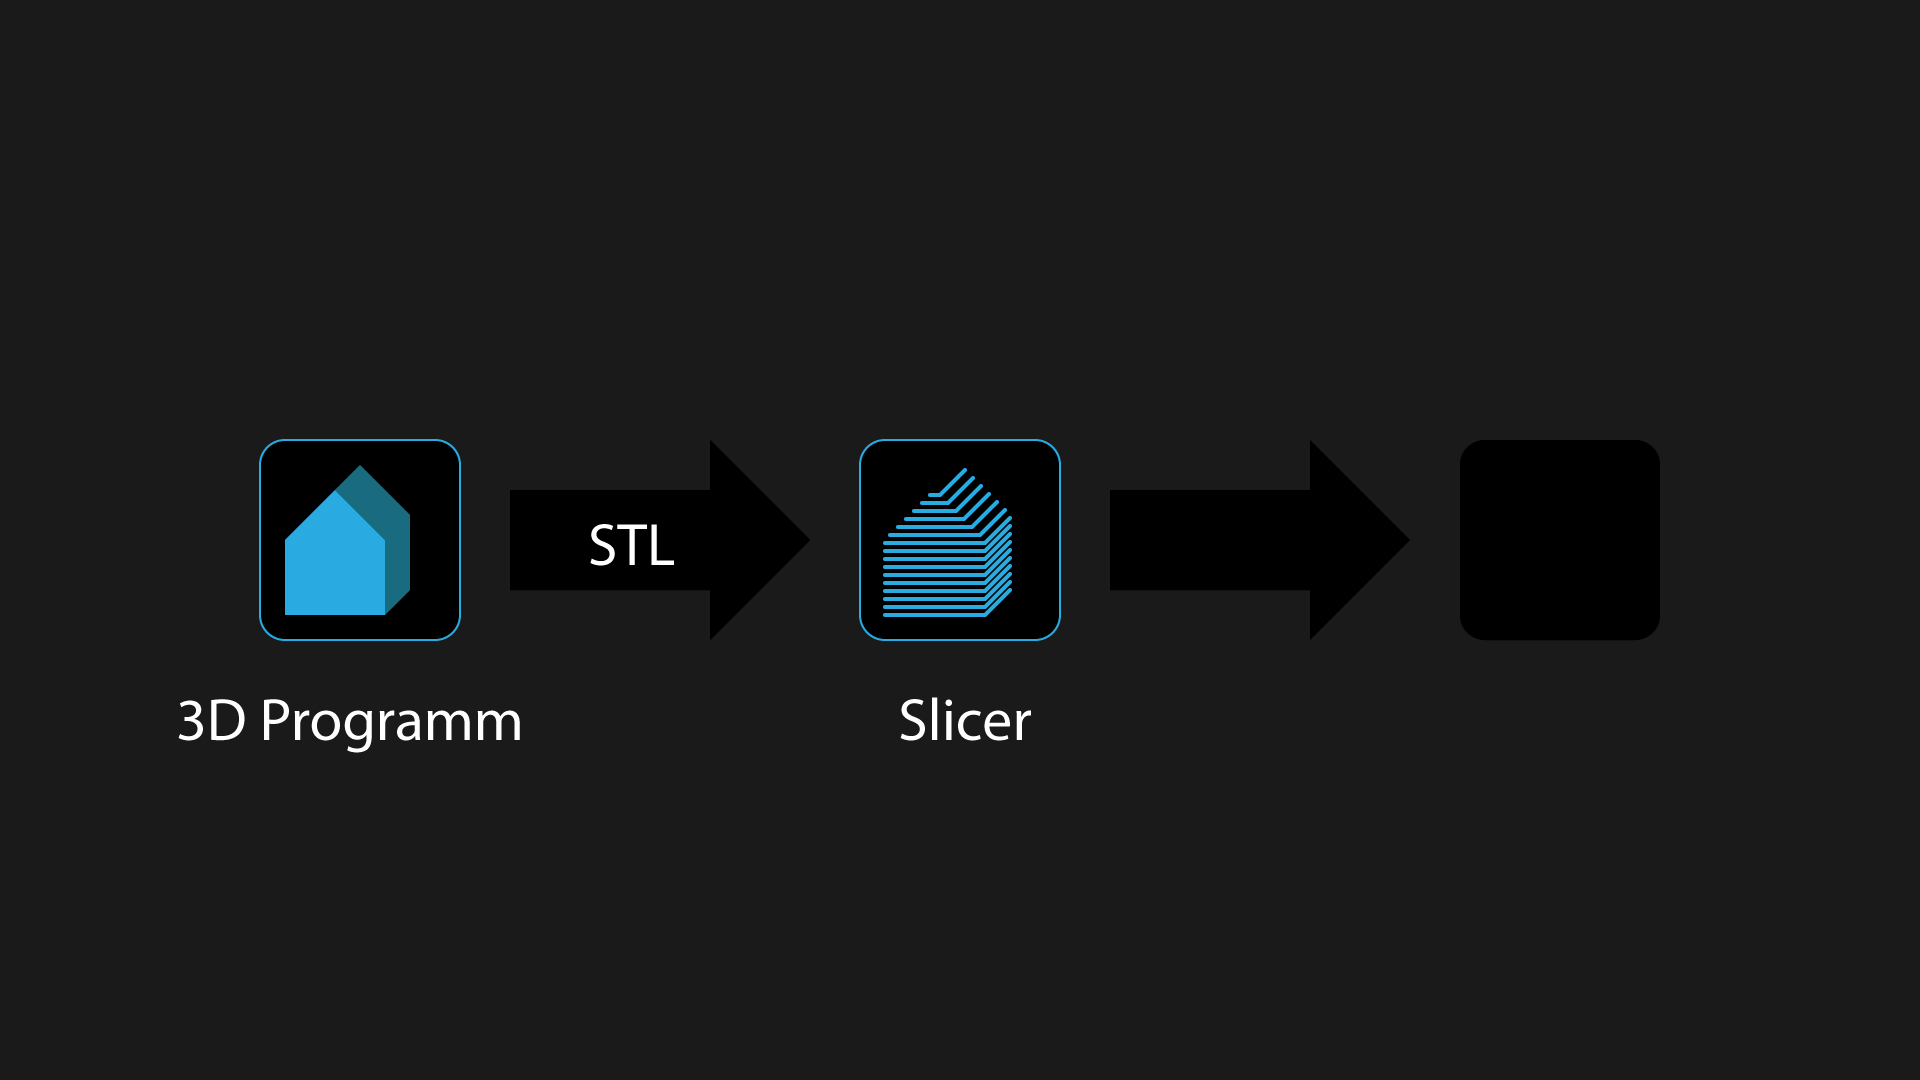
\includegraphics[width=\paperwidth]{images/steps/slicer.png}\hfil}\vfil}
}
}
\begin{frame}
  \frametitle{Slicer}
\end{frame}
}
{
\usebackgroundtemplate{%
\colorbox{BackgroundJGH}{%
\vbox to \paperheight{\vfil\hbox to \paperwidth{\hfil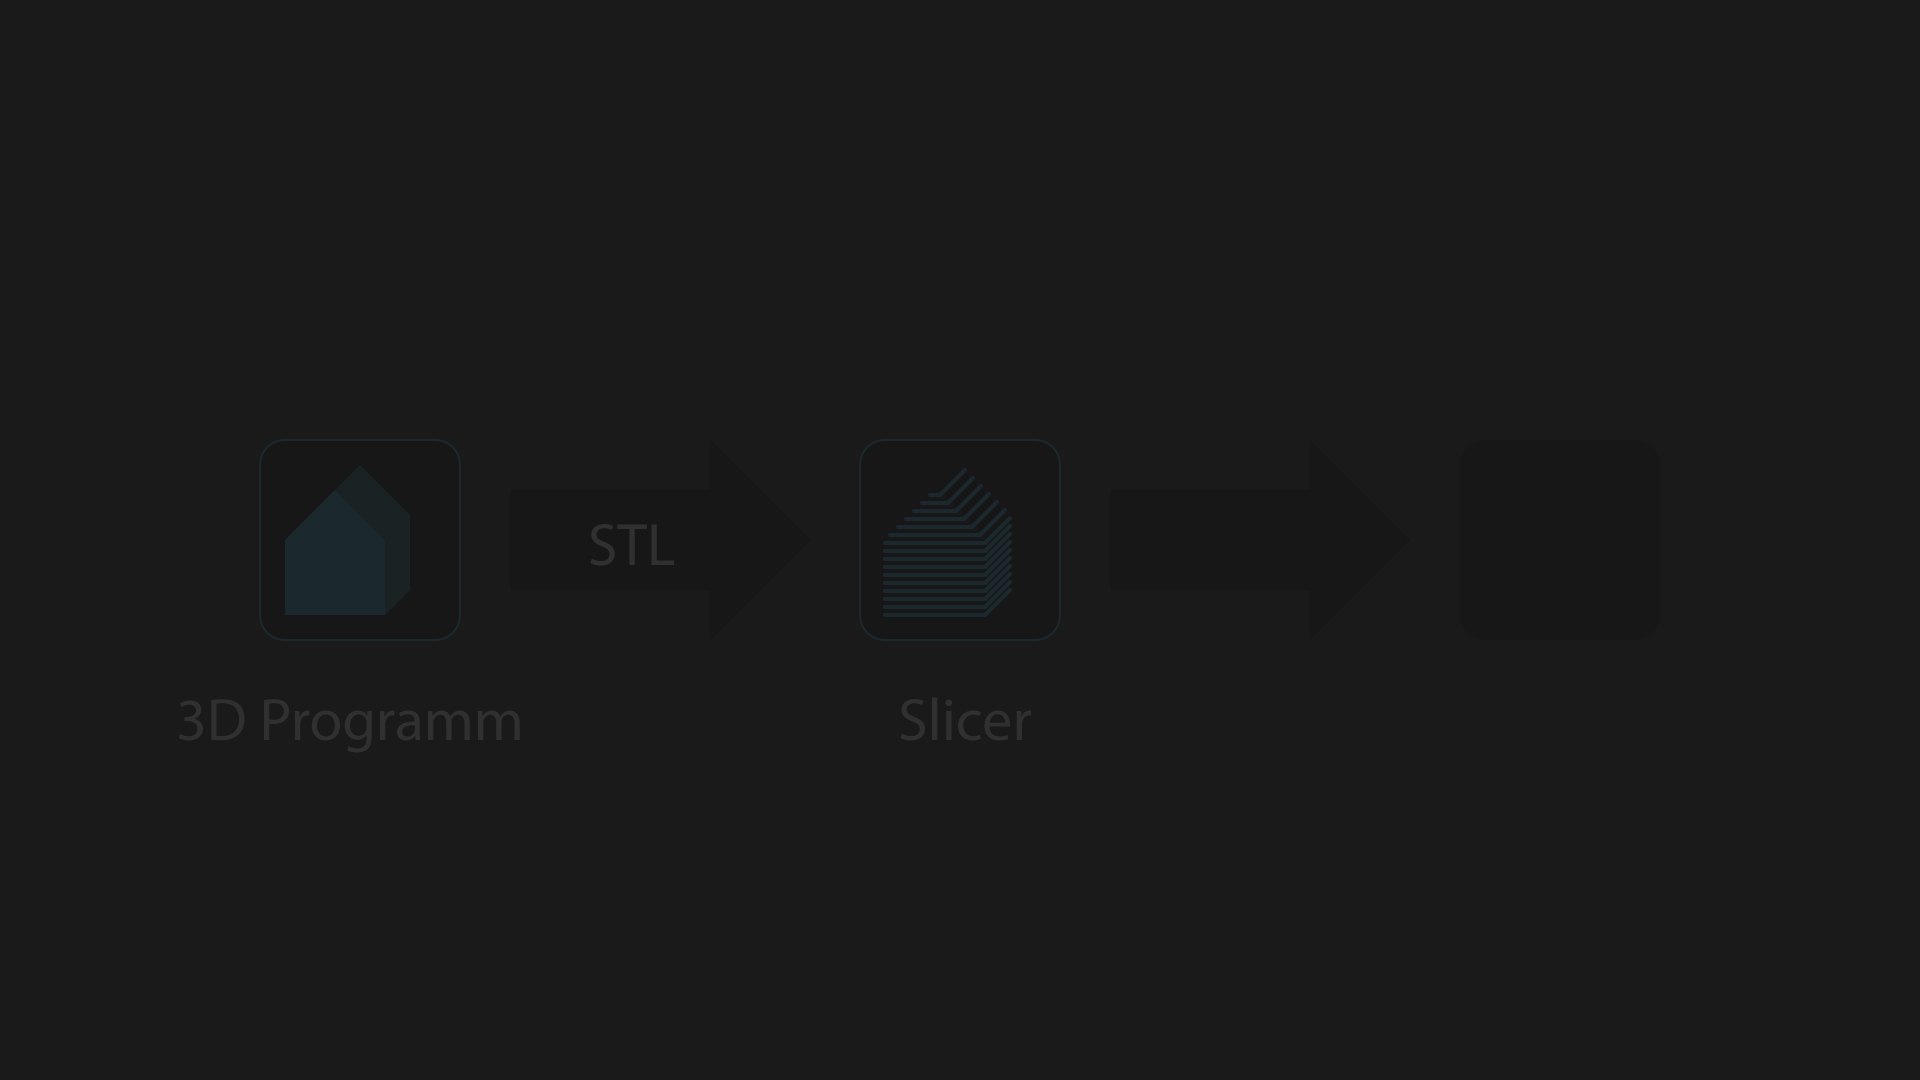
\includegraphics[width=\paperwidth]{images/steps/slicer_bg.png}\hfil}\vfil}
}
}
\begin{frame}
  \frametitle{Slicer}
  \begin{itemize}
    \item Vorbereitung für den Druck \pause
    \begin{itemize}
      \item Auswahl des Druckers \pause
      \item Platzieren auf dem Druckbett \pause
      \item Einstellen der Schichtdicke \pause
      \item Einstellen der Parameter für das Filament \pause
      \item Steuerkommandos für den jeweiligen Drucker
    \end{itemize}
  \end{itemize}
\end{frame}
}
{
\usebackgroundtemplate{%
\colorbox{BackgroundJGH}{%
\vbox to \paperheight{\vfil\hbox to \paperwidth{\hfil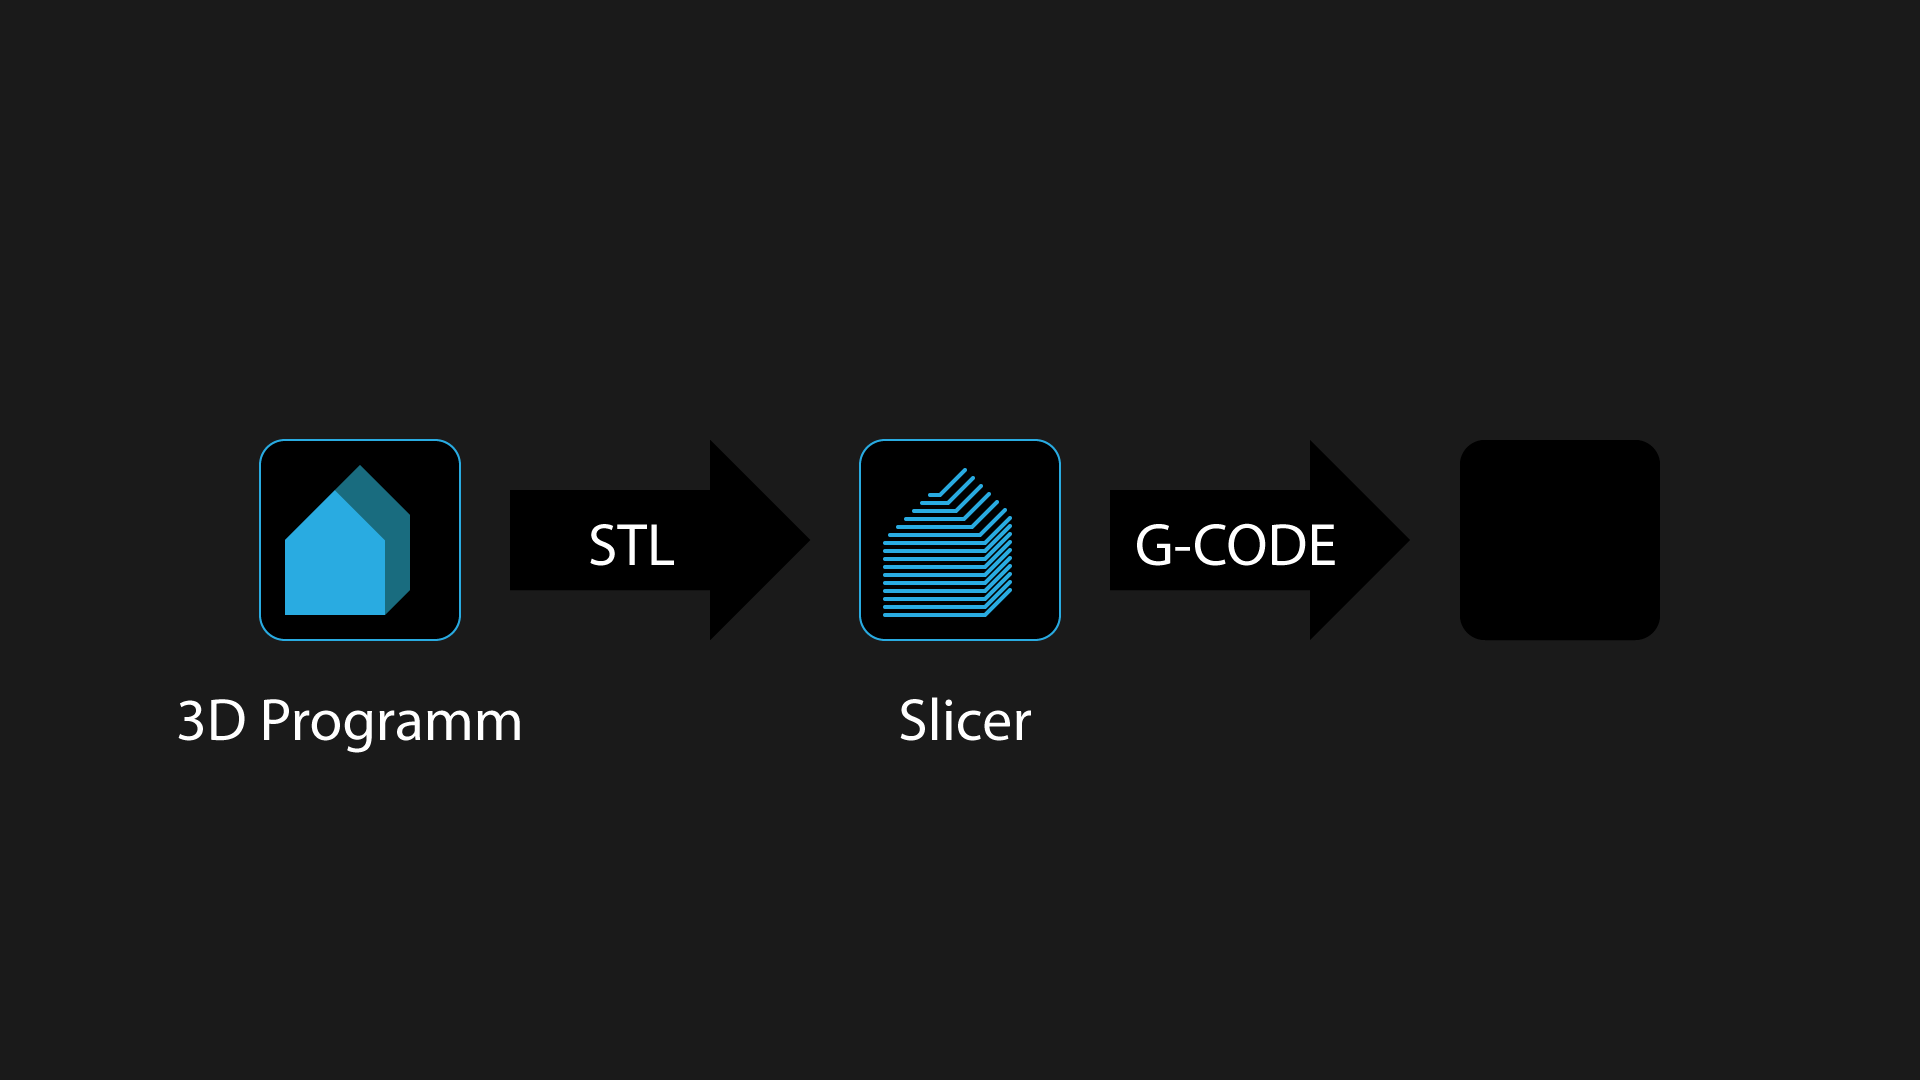
\includegraphics[width=\paperwidth]{images/steps/gcode.png}\hfil}\vfil}
}
}
\begin{frame}
  \frametitle{G-Code Datei}
\end{frame}
}
{
\usebackgroundtemplate{%
\colorbox{BackgroundJGH}{%
\vbox to \paperheight{\vfil\hbox to \paperwidth{\hfil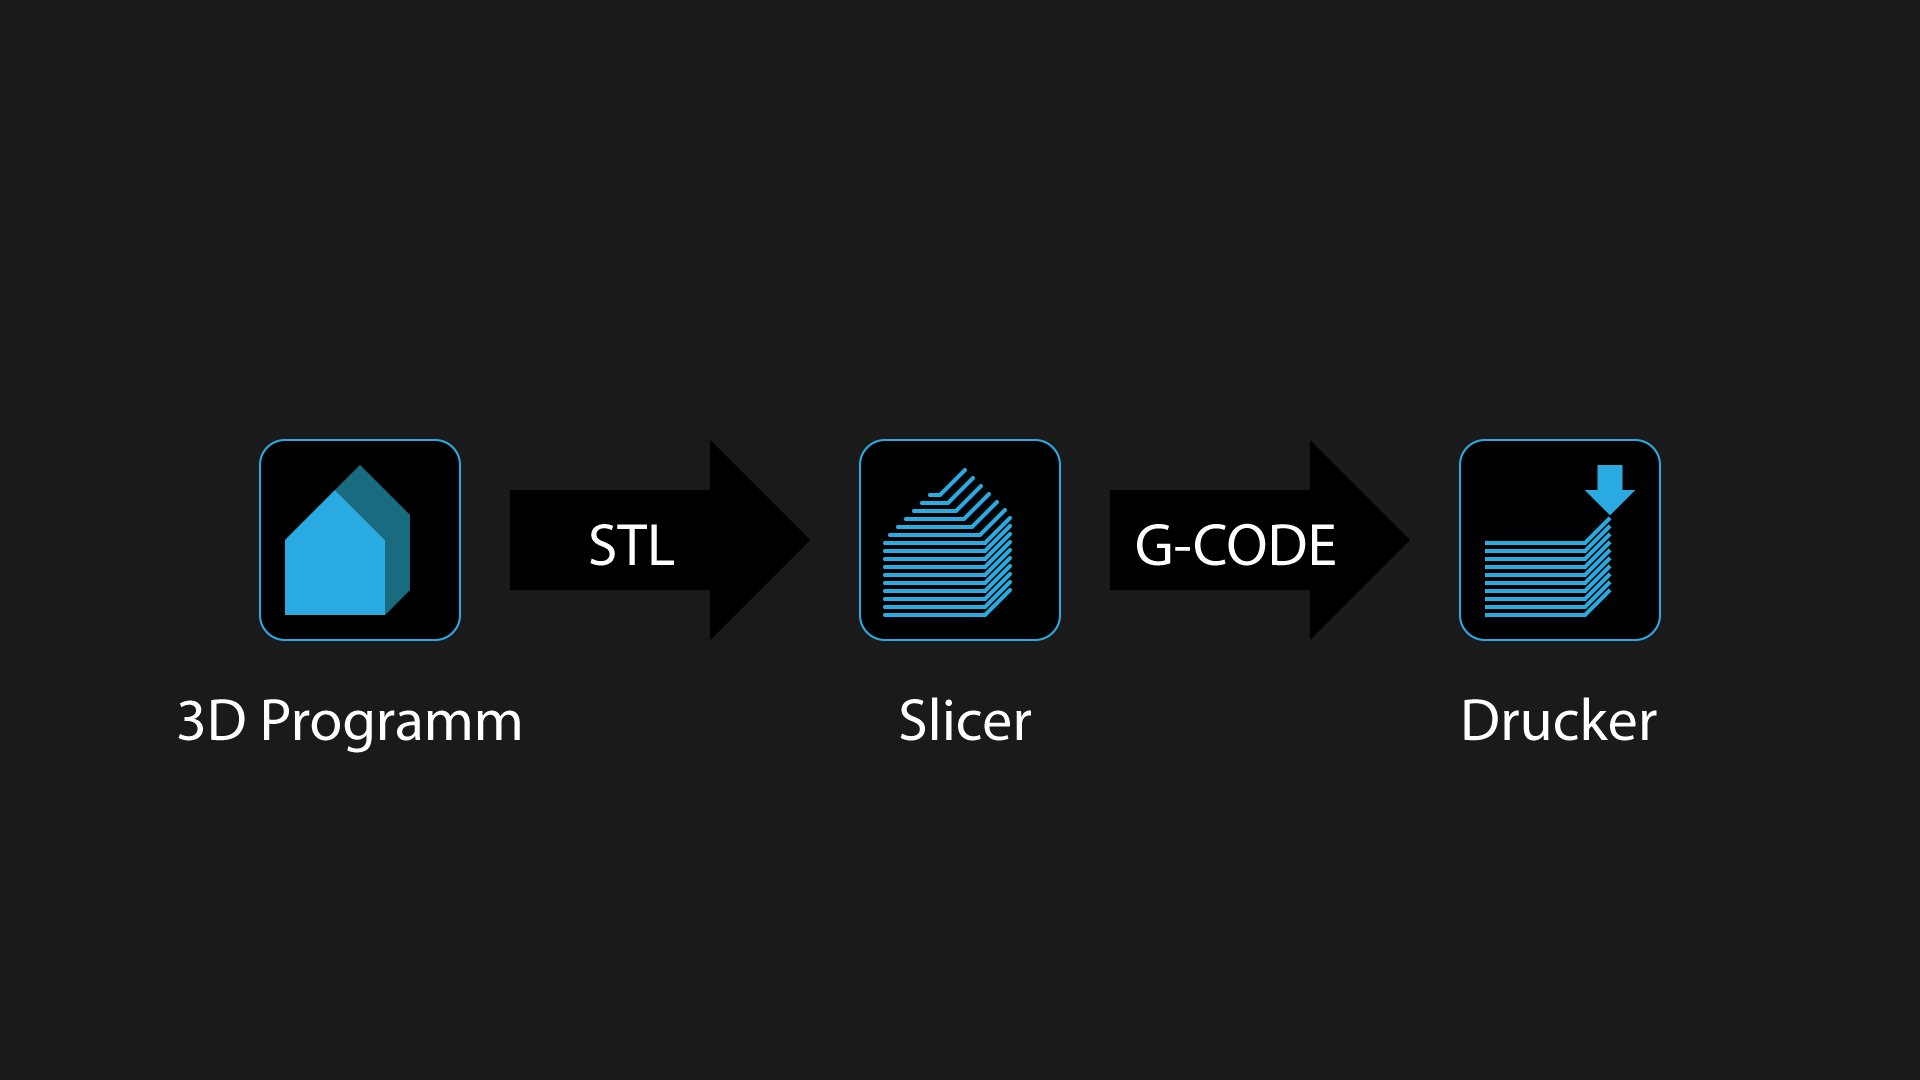
\includegraphics[width=\paperwidth]{images/steps/drucker.png}\hfil}\vfil}
}
}
\begin{frame}
  \frametitle{Drucker}
\end{frame}
}
{
\usebackgroundtemplate{%
\colorbox{BackgroundJGH}{%
\vbox to \paperheight{\vfil\hbox to \paperwidth{\hfil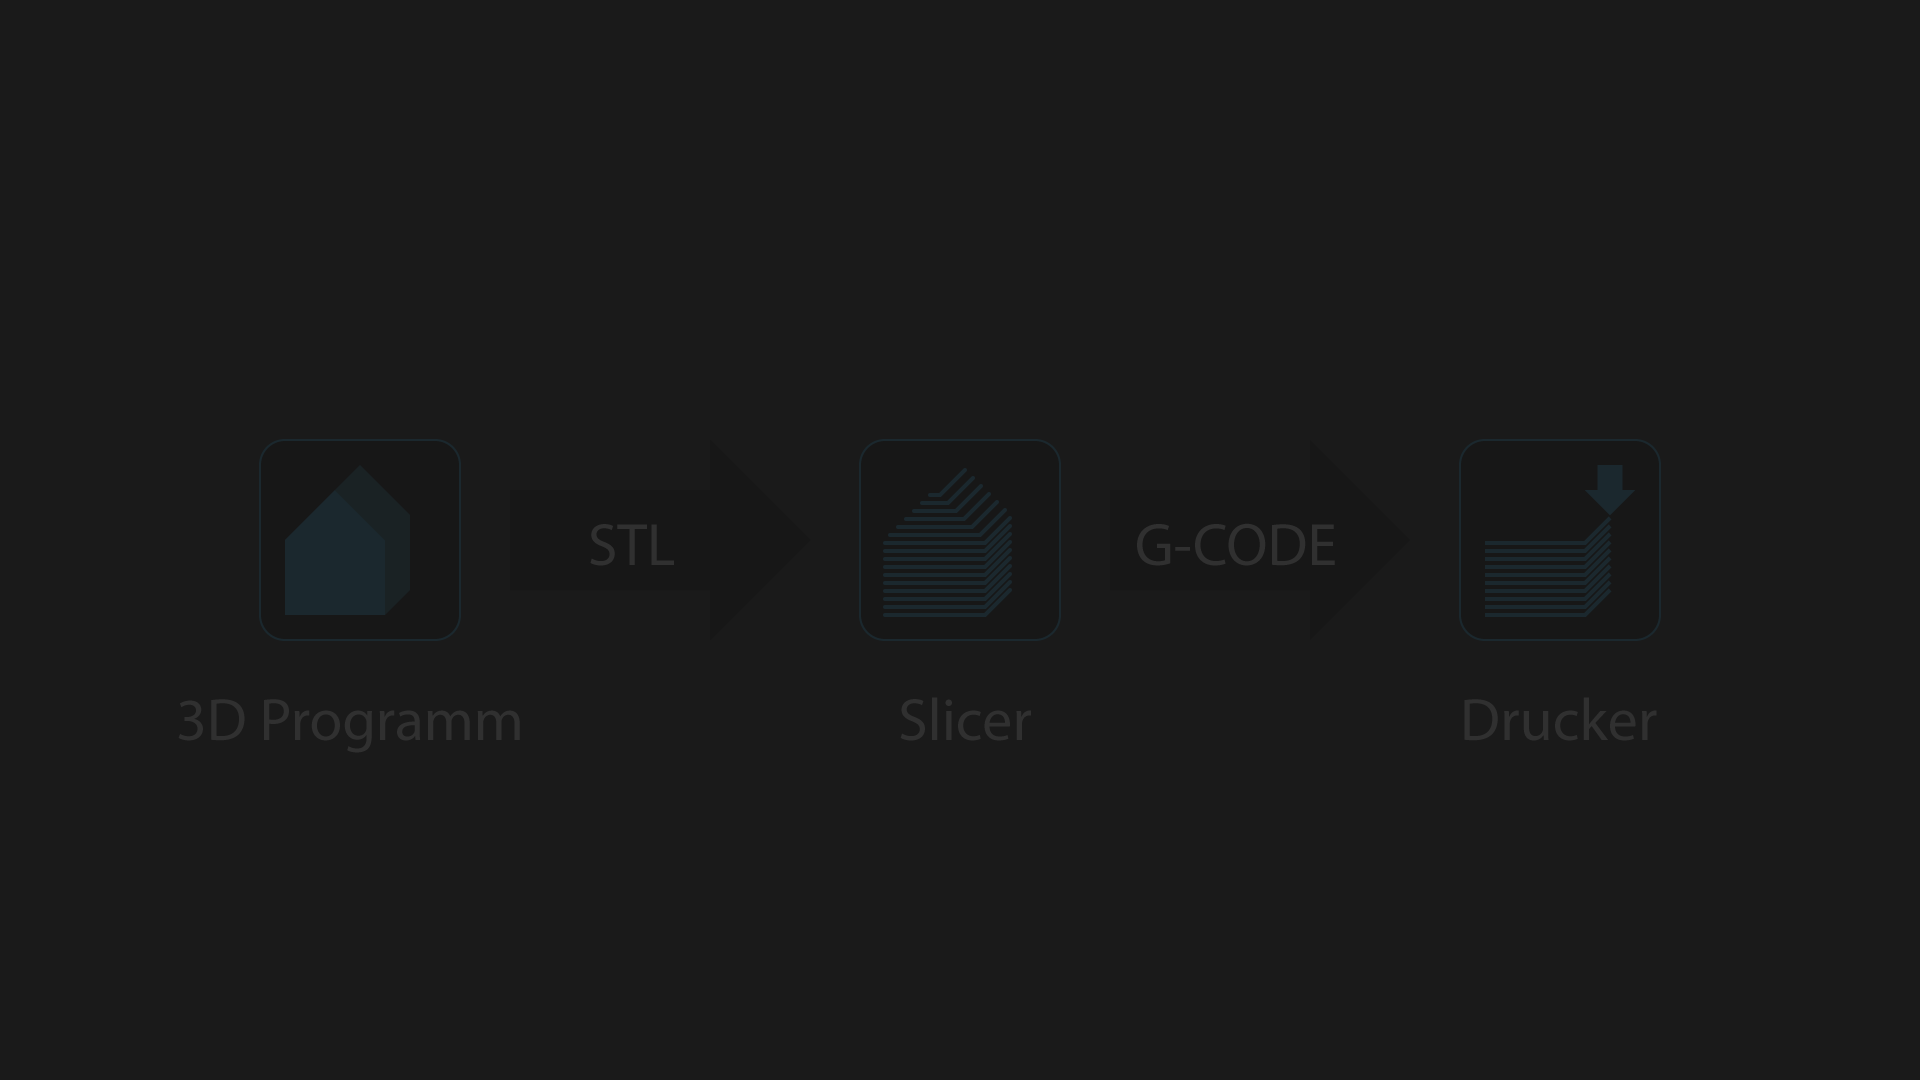
\includegraphics[width=\paperwidth]{images/steps/drucker_bg.png}\hfil}\vfil}
}
}
\begin{frame}
  \frametitle{Drucker}
  \begin{itemize}
    \item Übertragen der G-Code Datei \pause
    \begin{itemize}
      \item SD-Karte \pause
      \item USB-Stick \pause
      \item WiFi \pause
    \end{itemize}
    \item G-Code nur mit jeweiligem Drucker kompatibel \pause
    \begin{itemize}
      \item Vorsicht! Drucker kann kaputt gehen!
    \end{itemize}
  \end{itemize}
\end{frame}
}
